%% Glaukopis -- Computers & Security submission draft, v1.5 (2026-09-06).
%% Built from doc/v1.4 (abridged)/glaukopis_abridged_v1.4.tex after a
%% re-verification of every number against the results workbook, the
%% per-suite run manifests, the cost ledger code, the v21 build reports and
%% the per-item prediction artifacts (see REVISION_MEMORANDUM_v1.5.md).
%% Compile: bash build.sh   (pdflatex -> bibtex -> pdflatex x2)
\documentclass[preprint,12pt,authoryear]{elsarticle}
\usepackage[T1]{fontenc}
\usepackage{lmodern}
\usepackage{amsmath,amssymb}
\usepackage{booktabs,array,tabularx,multirow}
\usepackage{graphicx}
\usepackage{xcolor}
\usepackage{xurl}
\usepackage{tikz}
\usetikzlibrary{arrows.meta,positioning,fit,backgrounds,calc}
\usepackage{pgfplots}
\usepgfplotslibrary{groupplots}
%% compat=1.15 is the highest level accepted by the pgfplots 1.15 (2017) that
%% TexpadTeX/Texifier bundles; newer pgfplots (TeX Live ships 1.18.1) accepts it
%% too, so both toolchains render this figure identically. Do not raise it
%% without checking the version available in every build environment used.
\pgfplotsset{compat=1.15}
\usepackage{listings}
\usepackage{lineno}
\usepackage[hidelinks]{hyperref}
\modulolinenumbers[5]
\setlength{\emergencystretch}{2em}
\renewcommand{\topfraction}{0.95}
\renewcommand{\bottomfraction}{0.95}
\renewcommand{\textfraction}{0.03}
\renewcommand{\floatpagefraction}{0.75}
\setcounter{topnumber}{4}\setcounter{bottomnumber}{4}\setcounter{totalnumber}{8}
\lstset{basicstyle=\footnotesize\ttfamily,breaklines=true,columns=fullflexible,keepspaces=true,frame=single,showstringspaces=false}
\newcommand{\code}[1]{\path{#1}}
\newsavebox{\fitbox}
\newcommand{\fitwidth}[1]{\sbox{\fitbox}{#1}\ifdim\wd\fitbox>\textwidth\resizebox{\textwidth}{!}{\usebox{\fitbox}}\else\usebox{\fitbox}\fi}
\newcommand{\ci}[2]{{\scriptsize[#1,\,#2]}}
\newcommand{\Abal}{A_{\mathrm{bal}}}
\newcommand{\Bbal}{B_{\mathrm{bal}}}
\newcommand{\Tbal}{T_{\mathrm{bal}}}
\definecolor{seriesblue}{HTML}{2A78D6}
\definecolor{refgray}{HTML}{52514E}
%% ---------------------------------------------------------------------------
%% Compatibility shim for elsarticle < 3.0. \affiliation and the highlights
%% environment were introduced in elsarticle 3.x (TeX Live ships 3.3,
%% 2020/11/20). Older classes, such as the 1.2.0 (2009) copy bundled with
%% TexpadTeX/Texifier, leave both undefined, so their arguments are typeset
%% as raw text on a spurious first page and the affiliation labels never
%% resolve. When the class already defines them this block does nothing.
\makeatletter
\@ifundefined{affiliation}{%
  \RequirePackage{keyval}%
  \def\els@aff@text{}%
  \def\els@aff@add#1{%
    \ifx\els@aff@text\@empty\gdef\els@aff@text{#1}%
    \else\g@addto@macro\els@aff@text{, #1}\fi}%
  \define@key{els@aff}{organization}{\els@aff@add{#1}}%
  \define@key{els@aff}{addressline}{\els@aff@add{#1}}%
  \define@key{els@aff}{city}{\els@aff@add{#1}}%
  \define@key{els@aff}{postcode}{\els@aff@add{#1}}%
  \define@key{els@aff}{state}{\els@aff@add{#1}}%
  \define@key{els@aff}{country}{\els@aff@add{#1}}%
  \newcommand{\affiliation}[2][]{%
    \gdef\els@aff@text{}%
    \setkeys{els@aff}{#2}%
    \if\relax\detokenize{#1}\relax
      \edef\els@aff@tmp{\noexpand\address{\unexpanded\expandafter{\els@aff@text}}}%
    \else
      \edef\els@aff@tmp{\noexpand\address[#1]{\unexpanded\expandafter{\els@aff@text}}}%
    \fi
    \els@aff@tmp}%
}{}
\@ifundefined{highlights}{%
  \newbox\els@hlbox
  \def\els@prelimauthors{}%
  \let\els@author@orig\author
  \def\author{\@ifnextchar[{\els@author@opt}{\els@author@noopt}}%
  \def\els@author@opt[#1]#2{\els@prelimauthor{#2}\els@author@orig[#1]{#2}}%
  \def\els@author@noopt#1{\els@prelimauthor{#1}\els@author@orig{#1}}%
  \def\els@prelimauthor#1{\g@addto@macro\els@prelimauthors{\els@prelimsep#1}}%
  \newenvironment{highlights}{%
    \global\setbox\els@hlbox=\vbox\bgroup\hsize=\textwidth\def\baselinestretch{1}%
    \noindent{\Large Highlights}\par\vskip12pt
    \noindent\textbf{\@title}\par\vskip6pt
    \noindent{\let\corref\@gobble\let\fnref\@gobble\let\tnoteref\@gobble
      \def\els@prelimsep{\def\els@prelimsep{, }}\els@prelimauthors}\par\medskip
    \begin{itemize}}{\end{itemize}\egroup}%
  \let\els@maketitle@orig\maketitle
  \def\maketitle{%
    \ifvoid\els@hlbox\else
      \thispagestyle{empty}\unvbox\els@hlbox\clearpage\setcounter{page}{1}%
    \fi
    \els@maketitle@orig}%
}{}
\makeatother
%% ---------------------------------------------------------------------------
\journal{Computers \& Security}

\begin{document}
\begin{frontmatter}

\title{Glaukopis: Auditable Graph-Grounded Instruction Tuning for Cyber Threat Intelligence}

\author[fau,asg]{Peter J. Worth Jr.\corref{cor1}}
\ead{pworthjr@athenasecuritygrp.com}
\author[fau,asg]{Ionut Cardei}
\author[rai]{Salman Ahmad}
\author[rai]{Muhammad Mamoon Khan}
\cortext[cor1]{Corresponding author. ORCID: 0000-0003-4211-3866.}
\affiliation[fau]{organization={Department of Electrical Engineering and Computer Science, Florida Atlantic University},city={Boca Raton},state={FL},country={USA}}
\affiliation[asg]{organization={Athena Security Group, LLC},country={USA}}
\affiliation[rai]{organization={RevolveAI}}
%% TODO (authors): confirm the RevolveAI city/country and each author's ORCID before submission.

\begin{abstract}
Cyber threat intelligence (CTI) assistants must map free-text observations to security schemas, and the data used to specialize them must be open to inspection. Glaukopis addresses training-data traceability with Ariadne, a Neo4j graph integrating twelve public CTI sources, and Sophia, a template engine that materializes instruction targets by executing typed graph queries, so that every CTI target resolves to a graph binding and public-source identifiers. A four-stage supervised fine-tuning schedule on Qwen2.5-32B-Instruct retains a checkpoint after each stage for diagnosis. We re-derive every reported figure from the evaluation artifacts and correct the composite that earlier drafts used: under an explicit 50/50 blend of the two threat-attribution forms, the three-benchmark mean rises from 57.7 for the base model to 65.0 for the final checkpoint (95\% item-bootstrap interval 64.1--66.0). The gain is confined to the training-aligned AthenaBench tasks: attack-technique extraction improves from 18.2 to 65.8 and mitigation scoring from 7.6 to 62.5, while CyberSOCEval is unchanged, CyberMetric is flat, and MMLU-Pro falls by 11.6 points. Item-level audits show that the collapse of canonical attribution after the SOC-oriented stage is a semantic error rather than a format failure, that the severity-prediction regression concentrates in the exploitability metrics, and that exact gold-fact overlap between training rows and evaluation items does not inflate the mapping scores. We quantify n-gram and entity overlap, separate recorded evaluation expenditure from single-pass cost, and identify the training controls, repeated seeds, and independent incident sets still needed to claim scheduling advantages.
\end{abstract}

%% Highlights are uploaded to Elsevier as a separate file (highlights.txt in this
%% folder), so the environment below stays commented out: with elsarticle 3.x it
%% would typeset an extra unnumbered Highlights page before the title page.
%% Re-enable it only if a Highlights page inside the manuscript PDF is wanted.
%\begin{highlights}
%\item Sophia materializes CTI instruction targets by executing typed graph queries
%\item Retained checkpoints expose task interference hidden by a single final score
%\item Balanced attribution aggregation: 65.0 vs.\ 57.7 base, all gain in aligned tasks
%\item Item-level audit: attribution collapse is semantic, not a parsing artifact
%\item Gold-fact overlap, n-gram screening and cost accounting are quantified
%\end{highlights}

\begin{keyword}
cyber threat intelligence \sep instruction fine-tuning \sep knowledge graphs \sep data provenance \sep language-model evaluation \sep catastrophic interference
\end{keyword}

\end{frontmatter}

\linenumbers

\section{Introduction}\label{sec:intro}
Cyber threat intelligence (CTI) work connects vulnerability descriptions, weakness classes, attacker behaviors, and defensive actions. A language model may be fluent yet return a parent ATT\&CK technique instead of the requested sub-technique, select a related but incorrect CWE, or emit an unusable structured answer. CTIBench and AthenaBench make these distinctions operational through task-specific evaluation rather than relying only on general language-model benchmarks \citep{alam2024ctibench,alam2025athenabench}.

The deployment problem is not that every regulated organization is categorically prohibited from using external models. Rather, some security operations centers (SOCs) face contractual, confidentiality, data-residency, or infrastructure constraints that make locally served models preferable. Under those constraints, a practical question is whether specialization of an existing open-weight model improves the required CTI tasks without obscuring its training provenance or its losses on other workloads. This study targets a locally deployable 32-billion-parameter (32B) model; it does not establish a universal minimum model size or a compliance certification.

Glaukopis addresses two concrete engineering problems. First, instruction targets synthesized from unstructured material can be difficult to trace to a specific source fact. Sophia instead obtains the CTI target from an executed query over the Ariadne knowledge graph. Second, a single final model score hides when specialization introduces failures. Glaukopis retains checkpoints after Core, attribution-oriented (+TAA), SOC-oriented (CSE), and recalibration stages, exposing both improvements and regressions. The data pipeline is the central technical contribution. The stage sequence is an instrumented training configuration, not a demonstrated improvement over all single-stage alternatives.

The evidence also limits the claim. Training shards intentionally target the schemas used by the evaluation suites. Two of the authors (Worth and Ahmad) are co-authors of AthenaBench \citep{alam2025athenabench}; different data-generation pipelines therefore do not establish organizationally independent evaluation. The 32B final checkpoint improves several AthenaBench tasks, but it does not improve CyberSOCEval over the base and lowers general-task performance. Accordingly, the study asks whether graph-materialized instruction construction and checkpoint-level reporting provide a useful, inspectable CTI specialization workflow, not whether the model is a general-purpose SOC replacement.

This version of the study differs from the conference draft that preceded it in one important respect: every reported number has been re-derived from the primary artifacts. That audit found that the AthenaBench composite previously reported for the fine-tuned checkpoints used only the Classic attribution form while the hosted-reference rows used a 50/50 blend of the Classic and Canonical forms, and that the local rows of the evaluation-cost ledger counted every task twice. Both corrections are described in the body and change the headline values but not the qualitative findings. The audit also enabled analyses that the conference draft lacked: paired item-level bootstrap intervals across the retained checkpoints, an error taxonomy for the attribution collapse and the severity regression, quantified n-gram and gold-fact overlap between training and evaluation, and evaluation scores on overlapping versus non-overlapping items.

The contributions are: (i) a CTI data-construction architecture with graph-relative target provenance; (ii) an explicit multi-stage recipe and retained-checkpoint analysis of schema adaptation and interference, with item-level uncertainty and error taxonomies; (iii) a quantified contamination and alignment audit covering n-gram overlap, entity overlap, and gold-fact overlap; and (iv) a bounded evaluation that separates task scores, aggregation conventions, and cost-accounting assumptions. The public software is identified as a source-available artifact distinct from this article \citep{glaukopis2026software}. No superiority claim is made for stage ordering, graph-generated data versus a matched alternative, or lifecycle economics without the corresponding control.

\section{Problem formulation and scope}\label{sec:problem}
\subsection{Inputs, outputs, and provenance}
Let $G_t=(V_t,E_t,A_t)$ be a versioned CTI graph at snapshot $t$, comprising typed entities, relationships, and attributes. A template $\tau$ specifies a typed query $q_\tau$, constraints, and rendering functions. For a returned binding $b\in q_\tau(G_t)$, Sophia constructs
\begin{align}
 r_{\tau,b}&=\bigl(i_\tau(b),x_\tau(b),y_\tau(b)\bigr),\\
 y_\tau(b)&=\operatorname{render}_{\tau}\bigl(q_\tau(G_t),b\bigr).
\end{align}
Here $i$ is the instruction, $x$ the optional context or question, and $y$ the supervised target. An audit links the row to its template, graph snapshot, and bound public identifiers. In the released data these provenance elements are carried by the generation artifacts and by a per-row template identifier (\code{shortname}) and source tag; the three-field Alpaca training record alone does not encode a complete immutable provenance manifest.

The resulting model $p_\theta(y\mid i,x)$ is trained with ordinary next-token cross-entropy. For stage $s$ and its training set $D_s$, the objective is
\begin{equation}
 \mathcal{L}_s(\theta)=-\sum_{(i,x,y)\in D_s}\sum_{j=1}^{|y|}
 \log p_\theta(y_j\mid i,x,y_{<j}),
\end{equation}
with the preceding checkpoint initializing the next stage. No new optimizer, loss function, or inference architecture is introduced. Changes in data, order, sequence length, learning rate, and packing are all part of the observed treatment; a stage transition is not an isolated causal estimate of any one of them.

\subsection{Technical requirements and non-goals}
The system seeks source-resolvable supervision, controllable coverage of CTI schemas, inspectable specialization trade-offs, and local serving of the resulting checkpoint. These are distinguishable requirements. A target consistent with a stored graph can still be wrong because a source record is incomplete, a relationship is misinterpreted, or the graph is stale. Similarly, graph-grounded training does not guarantee graph-faithful model answers at inference time. Runtime constrained decoding, retrieval, or output verification would be separate mechanisms.

The evaluation concerns structured public-CTI tasks. It does not establish reliable handling of arbitrary private telemetry, autonomous containment, legal or regulatory interpretation, secure-code generation, or production incident attribution. For these workloads, a benchmark score is not an operational acceptance test. The deployed assistant should be constrained to validated task types, with schema checks, source verification, human approval, and abstention or escalation outside its evaluated scope.

\section{Background and related work}\label{sec:related}
\paragraph{Instruction fine-tuning}
Instruction fine-tuning adapts pretrained models using instruction--response examples. FLAN established transfer to unseen instruction-formulated tasks \citep{wei2022flan}; InstructGPT combined supervised demonstrations with preference-based training \citep{ouyang2022instructgpt}; and subsequent work studied scaling instruction mixtures \citep{chung2024flant5}. Domain-adaptive continued training motivates separating broad domain absorption from narrow task behavior \citep{gururangan2020dontstop}. These results motivate investment in instruction data, but they do not prove that Glaukopis's particular four-stage supervised schedule is superior to a matched mixed-data run.

\paragraph{Security-specific instruction data and models}
CyberPal.AI uses expert-driven cybersecurity instruction construction and provides the closest comparison for domain-specific supervision \citep{levi2025cyberpal}. Its follow-on examines expert small-language-model specialization with enriched reasoning data \citep{levi2025toward}. SEvenLLM studies bilingual CTI instruction data and evaluation \citep{ji2024sevenllm}. CyberBench provides a multi-task cybersecurity evaluation and adaptation framework \citep{liu2024cyberbench}. Table~\ref{tab:positioning} positions Glaukopis against the closest systems. Its distinguishing design is the explicit query-to-target path for Sophia-produced CTI records: a label is the deterministic rendering of a graph binding, not a model- or expert-authored explanation. This is a provenance property, not a measured assertion that every alternative has lower label quality.

\begin{table}[!htbp]
\centering\footnotesize
\caption{Positioning against the closest security instruction-tuning systems. ``Partial'' means that the cited system uses structured schemas, graph paths, or grounding traces for part of its pipeline but does not make every generated label the deterministic result of executing a typed graph query. Characterizations are taken from the cited papers.}\label{tab:positioning}
\begin{tabularx}{\textwidth}{@{}p{2.6cm}XXXX@{}}
\toprule
System & Graph-grounded targets & LLM-generated training text & Staged training with retained checkpoints & Provenance of a training label \\
\midrule
CyberPal.AI / SecKnowledge \citep{levi2025cyberpal} & Partial: schemas and graph paths for subsets & Yes: LLM augmentation with content grounding & Curriculum ordering; per-stage checkpoints not reported & Source and schema traces; explanations require evaluator trust \\
Toward cybersecurity-expert SLMs \citep{levi2025toward} & Partial: multi-step task grounding & Yes: enriched reasoning traces & Data-enrichment pipeline; stage effects not isolated & Enriched traces with expert steering \\
Glaukopis (this work) & Yes: typed Ariadne queries materialize every Sophia row & No for Sophia targets; auxiliary general mixtures are external & Yes: Core, +TAA, CSE, and recalibration checkpoints retained and evaluated & Row resolves to template, graph binding, and public-source keys \\
\bottomrule
\end{tabularx}
\end{table}

\paragraph{CTI knowledge graphs}
CTI knowledge graphs address a related but distinct problem. Open-CyKG constructs an open cyber-threat knowledge graph from unstructured reports \citep{sarhan2021opencykg}. Such extraction work concerns how facts enter a graph; Glaukopis primarily concerns how a populated graph is projected into instruction targets. Extraction quality and target-materialization quality should not be conflated. The defensible guarantee is that a Sophia target is materialized from its bound graph data, not that the entire software stack never uses language models.

\paragraph{Benchmarks and contamination}
The evaluation uses AthenaBench, CyberSOCEval, CyberMetric, and a separate MMLU-Pro diagnostic \citep{alam2025athenabench,deason2025cybersoceval,tihanyi2024cybermetric,wang2024mmlupro}. Verbatim $n$-gram screening of training data against evaluation items follows the 13-token overlap window that GPT-3 used for its benchmark-contamination analysis \citep{brown2020gpt3}; other open pretraining efforts instead remove documents with paragraph-level leakage from evaluation data \citep{groeneveld2024olmo}. We adopt the 13-gram window and report what it does and does not cover.

\section{Ariadne and Sophia: the data pipeline}\label{sec:data}
\subsection{Ariadne's source and refresh boundaries}
Ariadne is the populated Neo4j substrate. The reported configuration integrates twelve public CTI sources: ATT\&CK, ENGAGE, CAPEC, CWE, D3FEND, CVE, NVD, CISA KEV, FIRST EPSS, Sigma, ExploitDB, and PoC-in-GitHub \citep{strom2018mitre,mitreCWE,mitreCAPEC,mitreCVE}. The resulting graph is reported at approximately 280,000 nodes and 480,000 relationships. These are approximate snapshot sizes, not a statement that all public CTI is covered. Bounded catalogs are loaded in full, while several high-churn vulnerability and exploitation feeds are scoped to 2024 onward. Refresh behavior is source-dependent: EPSS and the current-year NVD feed are re-downloaded routinely, whereas other sources remain cached until an explicit refresh. Dataset freshness must therefore be assessed from the per-source versions and acquisition times used in a build. Construction follows dependencies: controlled vocabularies are loaded before vulnerability overlays and exploit references, and identifiers support idempotent graph population. Source keys alone are insufficient for exact replay if the corresponding source record or graph snapshot has changed.

\begin{figure}[!htbp]
\centering
\resizebox{\textwidth}{!}{%
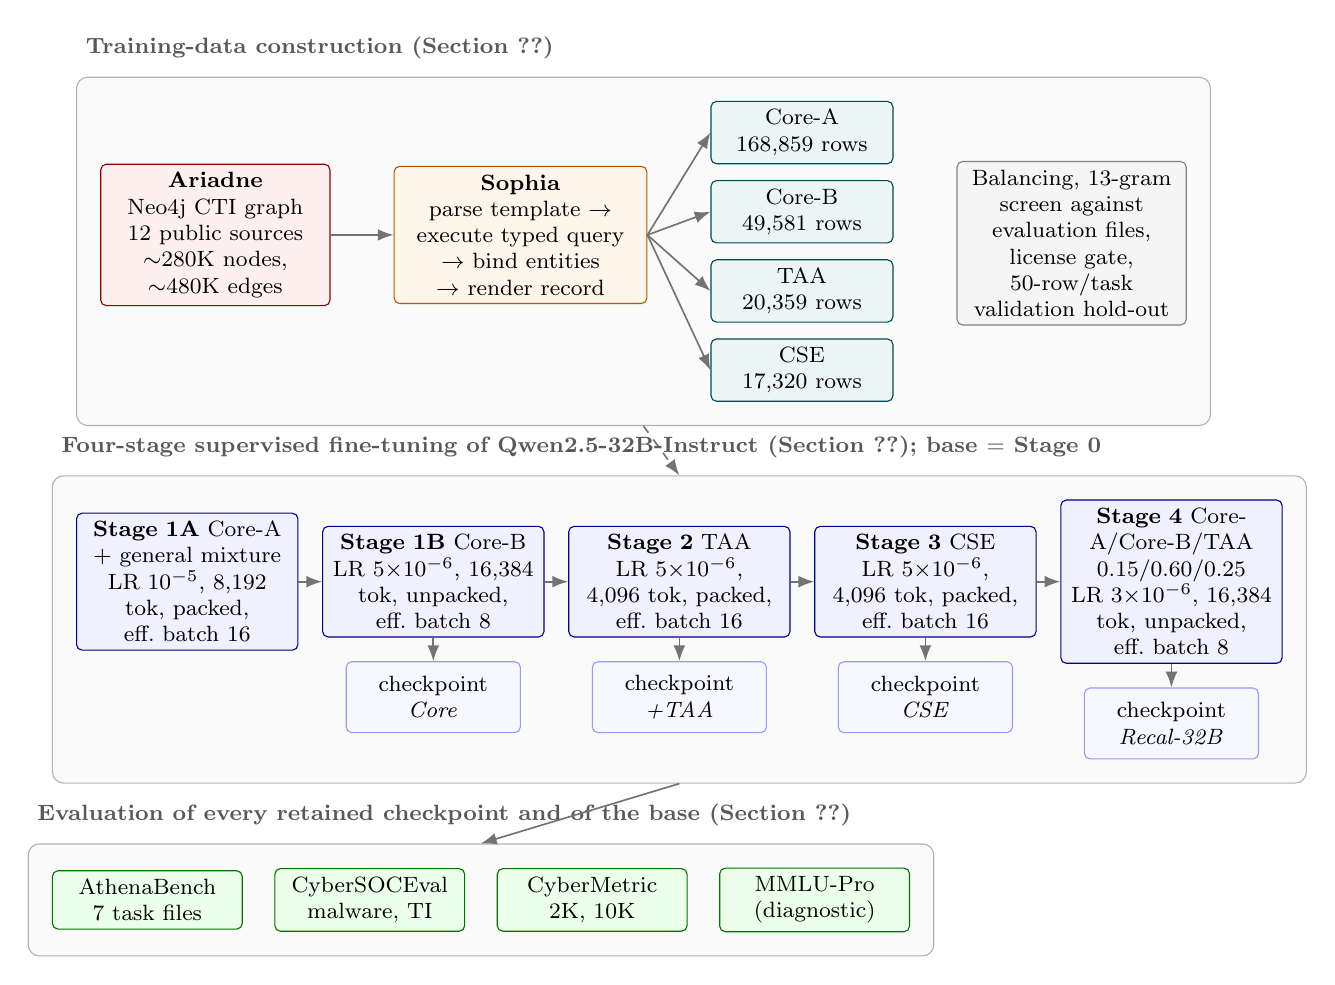
\begin{tikzpicture}[
  font=\footnotesize, >={Latex[length=2mm]}, node distance=3mm and 4mm,
  box/.style={draw, rounded corners=2pt, align=center, inner sep=3pt, minimum height=9mm},
  src/.style={box, fill=red!6, draw=red!55!black, text width=27mm},
  gen/.style={box, fill=orange!8, draw=orange!70!black, text width=30mm},
  shard/.style={box, fill=teal!8, draw=teal!60!black, text width=21mm, minimum height=7mm},
  stage/.style={box, fill=blue!6, draw=blue!55!black, text width=26mm},
  ev/.style={box, fill=green!8, draw=green!45!black, text width=22mm, minimum height=7mm},
  arr/.style={->, semithick, black!55}, grp/.style={draw=black!30, rounded corners=4pt, inner sep=3mm, fill=black!2},
  lbl/.style={font=\footnotesize\bfseries, text=black!65}]
\node[src] (ari) {\textbf{Ariadne}\\Neo4j CTI graph\\12 public sources\\$\sim$280K nodes, $\sim$480K edges};
\node[gen, right=8mm of ari] (sop) {\textbf{Sophia}\\parse template $\to$ execute typed query $\to$ bind entities $\to$ render record};
\node[shard, right=8mm of sop, yshift=13mm] (sa) {Core-A\\168,859 rows};
\node[shard, below=2mm of sa] (sb) {Core-B\\49,581 rows};
\node[shard, below=2mm of sb] (st) {TAA\\20,359 rows};
\node[shard, below=2mm of st] (sc) {CSE\\17,320 rows};
\node[box, fill=black!4, draw=black!50, text width=27mm, right=8mm of sb, yshift=-4mm] (scr) {Balancing, 13-gram screen against evaluation files, license gate, 50-row/task validation hold-out};
\draw[arr] (ari) -- (sop);
\foreach \s in {sa,sb,st,sc} \draw[arr] (sop.east) -- (\s.west);
\begin{scope}[on background layer]
 \node[grp, fit=(ari)(sop)(sa)(sc)(scr)] (g1) {};
\end{scope}
\node[lbl, above=1mm of g1.north west, anchor=south west] {Training-data construction (Section~\ref{sec:data})};
% stages
\node[stage, below=11mm of g1.south west, anchor=north west] (s1) {\textbf{Stage 1A} Core-A + general mixture\\LR $10^{-5}$, 8,192 tok, packed, eff.\ batch 16};
\node[stage, right=3mm of s1] (s1b) {\textbf{Stage 1B} Core-B\\LR $5{\times}10^{-6}$, 16,384 tok, unpacked, eff.\ batch 8};
\node[stage, right=3mm of s1b] (s2) {\textbf{Stage 2} TAA\\LR $5{\times}10^{-6}$, 4,096 tok, packed, eff.\ batch 16};
\node[stage, right=3mm of s2] (s3) {\textbf{Stage 3} CSE\\LR $5{\times}10^{-6}$, 4,096 tok, packed, eff.\ batch 16};
\node[stage, right=3mm of s3] (s4) {\textbf{Stage 4} Core-A/Core-B/TAA 0.15/0.60/0.25\\LR $3{\times}10^{-6}$, 16,384 tok, unpacked, eff.\ batch 8};
\draw[arr] (s1) -- (s1b); \draw[arr] (s1b) -- (s2); \draw[arr] (s2) -- (s3); \draw[arr] (s3) -- (s4);
\node[box, fill=blue!3, draw=blue!40, text width=20mm, below=3mm of s1b] (c1) {checkpoint\\\emph{Core}};
\node[box, fill=blue!3, draw=blue!40, text width=20mm, below=3mm of s2] (c2) {checkpoint\\\emph{+TAA}};
\node[box, fill=blue!3, draw=blue!40, text width=20mm, below=3mm of s3] (c3) {checkpoint\\\emph{CSE}};
\node[box, fill=blue!3, draw=blue!40, text width=20mm, below=3mm of s4] (c4) {checkpoint\\\emph{Recal-32B}};
\draw[arr] (s1b) -- (c1); \draw[arr] (s2) -- (c2); \draw[arr] (s3) -- (c3); \draw[arr] (s4) -- (c4);
\begin{scope}[on background layer]
 \node[grp, fit=(s1)(s4)(c1)(c4)] (g2) {};
\end{scope}
\node[lbl, above=1mm of g2.north west, anchor=south west] {Four-stage supervised fine-tuning of Qwen2.5-32B-Instruct (Section~\ref{sec:training}); base $=$ Stage 0};
% eval
\node[ev, below=11mm of g2.south west, anchor=north west] (e1) {AthenaBench\\7 task files};
\node[ev, right=4mm of e1] (e2) {CyberSOCEval\\malware, TI};
\node[ev, right=4mm of e2] (e3) {CyberMetric\\2K, 10K};
\node[ev, right=4mm of e3] (e4) {MMLU-Pro\\(diagnostic)};
\begin{scope}[on background layer]
 \node[grp, fit=(e1)(e4)] (g3) {};
\end{scope}
\node[lbl, above=1mm of g3.north west, anchor=south west] {Evaluation of every retained checkpoint and of the base (Section~\ref{sec:evaluation})};
\draw[arr] (g2.south) -- (g3.north);
\draw[arr, dashed] (g1.south) -- (g2.north);
\end{tikzpicture}}
\caption{Glaukopis pipeline as configured for the reported v21 release. Shard sizes are the realized post-screen training rows; stage settings are read from the release launchers. The general mixture in Stage 1A (T\"ulu-3 SFT and Alpaca) is not Sophia-generated and is not screened against the evaluation files.}\label{fig:pipeline}
\end{figure}

\begin{table}[!htbp]
\centering\footnotesize
\caption{Pipeline boundaries. Provenance is strongest for Sophia-materialized CTI targets; it should not be generalized to all auxiliary data or to unconstrained model completions.}\label{tab:boundaries}
\begin{tabularx}{\textwidth}{@{}p{2.4cm}XXX@{}}
\toprule Component & Input and transformation & Resulting artifact & Scope of assurance \\\midrule
Ariadne & Public CTI records normalized to typed entities and relations & Neo4j CTI snapshot & Source-linked facts; not proof of source completeness or correctness \\
Sophia & Expert-authored template, typed query, graph binding, rendering & Instruction, context, and target record with template identifier & Target traceable to the executed graph binding \\
Corpus preparation & Generation, balancing, $n$-gram screening, license gate, phase splitting & Core-A, Core-B, TAA, CSE, and validation shards & Dependent on covered files, fields, thresholds, and retained reports \\
Supervised training & Stage-specific shard mixture and optimizer configuration & Core, +TAA, CSE, Recal-32B checkpoints & Observable transitions; no isolated scheduling effect \\
Evaluation & Fixed task inputs, checkpoint, parser and scorer, serving settings & Predictions, per-item scores, run manifests & Reproducible only to the extent the run manifests and artifacts are retained \\\bottomrule
\end{tabularx}
\end{table}

\subsection{Typed-query materialization}
Sophia parses a declarative template, executes its typed graph query, binds the returned entities and relationships, and renders instruction records (Figure~\ref{fig:pipeline}). Templates support property access, relationship traversals, list expansion, hidden bindings, source disambiguation, and equality or inequality constraints. The following abbreviated pattern correlates a CVE with its weakness and attack pattern:
\begin{lstlisting}
Question: Correlate CVE, CWE, and CAPEC for a single vulnerability chain.
Answer: CVE {cve:CVE.id} impacts CAPEC {cap:cve.impacts>CAPEC.name}
and is categorized as weakness {cwe:cve.problemType>Weakness.name}.
CAPEC {cap.id} exploits weakness {cwe2:cap.exploits>Weakness.name}.
<*{force cwe.id=cwe2.id}*>
\end{lstlisting}
The hidden equality constraint requires the two traversals to resolve to the same weakness identifier. A reviewer can therefore inspect the binding rather than trust a separately synthesized answer. The example illustrates the materialization mechanism; it is not a new reasoning benchmark.

Negative constraints can generate examples that distinguish graph-supported from unsupported associations. However, absence of a relationship in an incomplete CTI graph is not necessarily evidence that the relationship is false in the world. Negative examples should be interpreted against the declared graph and schema, with a documented closed-world assumption where appropriate.

The generation workflow parses template manifests, materializes bindings, balances and deduplicates records, and serializes Alpaca-format JSON. Schema tests detect template references to absent graph labels, relationships, or properties. These tests can reveal incompatibilities but do not replace a semantic audit of source mappings. The combination provides content control and inspectability without establishing a measured reduction in all types of label error.

\subsection{Corpus scope and reproducibility}
The reported v21 release uses four production CTI shards (Core-A, Core-B, TAA, and CSE) and three validation shards holding out 50 rows per template family. The build reports record the realized sizes: the Core corpus contained 219,675 rows after balancing, of which 684 were removed by the $n$-gram screen (Section~\ref{sec:contamination}), 550 were held out for validation, and of the remaining 218,441 training rows 168,859 were assigned to Core-A and 49,581 to Core-B (the phase-split report accounts for all but one row); the TAA and CSE shards contained 20,359 and 17,320 training rows. Core-A is trained together with a general-purpose instruction mixture (T\"ulu-3 SFT and Alpaca-English; \citealp{lambert2024tulu3,taori2023alpaca}), which is neither Sophia-generated nor screened. Consequently, the statement ``every training example is graph-materialized'' applies to Sophia-generated CTI records only.

The architecture ports use the same serialized CTI release. Nevertheless, exact row-level regeneration was not fully seed-pinned in v21: graph-read order, sampling, and deduplication tie-breaks can vary, and the project's own replay experiments found that byte-identical templates did not reproduce per-task scores within the intended tolerance. Template identity alone therefore does not certify identical training rows. A reproducible release needs hashes of the serialized files, per-source graph snapshots, counts after each filter, and software versions, in addition to the templates.

\section{Multi-stage training configuration}\label{sec:training}
The canonical base is \code{Qwen/Qwen2.5-32B-Instruct} \citep{qwen2025qwen25}. Additional ports use Qwen2.5-14B-Instruct, Qwen3-30B-A3B-Thinking-2507, Meta-Llama-3.1-8B-Instruct, and Foundation-Sec-8B-Instruct. The mixture-of-experts (MoE) port should be distinguished by total and active parameter counts (30.5B total, 3.3B active per token).

Table~\ref{tab:training} states the schedule as read from the release launchers. Stage 1 has two phases. Core-A mixes broad CTI instruction families with the auxiliary general instructions; Core-B targets the RMS, ATE, VSP, and RCM schema tasks. Stage 2 specializes on threat-actor-attribution records. Stage 3 uses SOC-style structured-response drills. Stage 4 revisits earlier shards to seek a different capability balance. These are intended objectives; whether they are achieved is an empirical question. Training uses LlamaFactory \citep{zheng2024llamafactory} with DeepSpeed ZeRO-3 and CPU offload \citep{rajbhandari2020zero}, an 8-bit AdamW optimizer, Liger kernels, gradient checkpointing, and bfloat16 precision on eight 80-GB H100 GPUs. Effective batch size is preserved by adjusting gradient accumulation to the GPU count.

\begin{table}[!htbp]
\centering\footnotesize
\caption{Canonical 32B training recipe read from the v21 launchers. Caps are the per-dataset \texttt{max\_samples} limits, not realized token counts. The general mixture is capped separately from Core-A because the limit applies per dataset. Wall-time budgets are the project's documented planning figures for eight H100 GPUs, not metered bills of the reported runs.}\label{tab:training}
\fitwidth{\begin{tabular}{@{}llrrrrll@{}}
\toprule Pass & Training input & Cap & Max.\ tokens & LR & Eff.\ batch & Packing & Budget (h) \\\midrule
1A & Core-A + T\"ulu-3 SFT + Alpaca & 240,000 & 8,192 & $1\times10^{-5}$ & 16 & on & \multirow{2}{*}{26--30} \\
1B & Core-B & 70,000 & 16,384 & $5\times10^{-6}$ & 8 & off & \\
2 & TAA & 33,000 & 4,096 & $5\times10^{-6}$ & 16 & on & 13--17 \\
3 & CSE & 33,000 & 4,096 & $5\times10^{-6}$ & 16 & on & 9--13 \\
4 & Core-A/Core-B/TAA at 0.15/0.60/0.25 & 3,600 per shard & 16,384 & $3\times10^{-6}$ & 8 & off & 3--4 \\\bottomrule
\end{tabular}}
\end{table}

Because the caps exceed the realized Core-B, TAA, and CSE shard sizes, those passes consume their shards in one epoch. In pass 1A the cap applies to the Sophia shard and to each auxiliary dataset separately, so the general mixture can contribute up to 240,000 rows alongside the 168,859 Core-A rows; the auxiliary share is therefore material to the forgetting discussion in Section~\ref{sec:results}. Stage 4 interleaves the three shards under the stated probabilities up to the per-shard cap, which yields about 6,000 interleaved examples. Neither repeated exposure nor actual token consumption can be inferred from the caps; sequence limits are maxima, not average lengths.

The alternative Stage-4 recipe developed for the 14B port uses learning rate $10^{-6}$, mixture probabilities 0.25/0.40/0.35, and a 2,400-example cap. Both Stage-4 variants were trained from the same CSE parent on the 32B base and both are evaluated below. Applying different Stage-4 mixtures and rates across architectures means that the complete training treatment is not byte-identical across every port.

We call the retained models \emph{cumulative checkpoints}. They reveal the effects of continuing training under each configured treatment; they are not matched ablations. In particular, Core$\rightarrow$CSE without TAA and a one-stage mixture with matched realized tokens and updates were not run. The necessity of Stage 2 and the superiority of four stages are therefore unresolved.

\section{Evaluation protocol}\label{sec:evaluation}
\subsection{Task portfolio, scorers, and run records}
AthenaBench evaluates CTI knowledge (CKT), attack-technique extraction (ATE), root-cause mapping (RCM), risk-mitigation strategy (RMS), vulnerability-severity prediction (VSP), and threat-actor attribution (TAA) in Classic and Canonical forms \citep{alam2025athenabench}. CyberSOCEval supplies malware-analysis and threat-intelligence-reasoning tasks \citep{deason2025cybersoceval}; CyberMetric supplies cybersecurity multiple-choice evaluation at the 2K and 10K tiers \citep{tihanyi2024cybermetric}; MMLU-Pro is a general-task diagnostic \citep{wang2024mmlupro}. Table~\ref{tab:portfolio} lists the item counts and the scorer that the harness applies to each task, read from the evaluation code. The scorers differ in kind, so task scores should not all be called accuracy or treated as calibrated probabilities of operational success.

\begin{table}[!htbp]
\centering\footnotesize
\caption{Evaluation portfolio as executed for the 32B chain. Item counts are from the run manifests; scorer definitions are from the evaluation code. TAA and RMS ``combined'' scores award full credit for a strict match and half credit for a plausible match (an alias or related group for TAA; a mitigation from the technique's neighbourhood for RMS).}\label{tab:portfolio}
\begin{tabularx}{\textwidth}{@{}lrX@{}}
\toprule Task & Items & Per-item score used in the aggregates \\\midrule
CKT (multiple choice) & 3,000 & 1 if the option letter matches \\
RCM & 2,000 & 1 if the CWE identifier matches exactly \\
VSP & 2,000 & $1-|s_{\text{pred}}-s_{\text{gold}}|/7.7$, with $s$ the CVSS v3.1 base score of the parsed vector \citep{first2019cvss}; unparseable vectors are excluded (two of 2,000 for the final checkpoint) \\
ATE & 500 & 1 if the technique matches at the parent-technique level (sub-technique suffix ignored) \\
RMS & 500 & Set F1 over predicted mitigation identifiers; combined variant credits neighbourhood mitigations at half weight \\
TAA Classic & 100 & 1 alias-connected, 0.5 related group, 0 otherwise \\
TAA Canonical & 133 & 1 if the canonical group name or G-code appears, 0.5 if another alias of the group appears, 0 otherwise \\
CyberSOCEval malware / TI & 609 / 588 & Jaccard similarity between predicted and gold option-letter sets; strict accuracy is Jaccard $=1$; unparseable responses are excluded from both denominators \\
CyberMetric 2K / 10K & 2,000 / 10,180 & 1 if the option letter matches \\
MMLU-Pro & 12,032 & 1 if the extracted option letter matches (zero-shot chain-of-thought prompt) \\\bottomrule
\end{tabularx}
\end{table}

Local checkpoints were served with vLLM \citep{kwon2023vllm} on two H100 GPUs at batch size 32 (64 for MMLU-Pro), and hosted references used the same harness through provider APIs \citep{glaukopis2026software}. The run manifests date the CTI evaluations of the five 32B checkpoints to 20--21 May 2026 and the MMLU-Pro evaluations to 23--26 May 2026; the results workbook that collects them is dated 24 June 2026. Each score is a single evaluation of a single training run. Item-level prediction and score files were retained for the five fine-tuned checkpoints and are the basis of the bootstrap and error analyses below; the corresponding files for the base model and the hosted references were not available for this audit, so paired statistics involving them are not reported.

\subsection{Alignment between training shards and evaluation tasks}
Alignment is deliberate. Core-B trains the schemas assessed by AthenaBench's mapping and mitigation tasks; Stage 2 targets attribution; Stage 3 targets SOC-style answer formats; and Core-A includes CyberMetric-style and multiple-choice families. None of the three CTI benchmark families is a demonstrably untouched evaluation target. Sharing public catalogs is appropriate for measuring public-catalog competence, but it does not establish generalization to unseen facts, new incidents, or private SOC telemetry. Independent construction is not equivalent to entity-disjoint, fact-disjoint, or temporally held-out evaluation.

\subsection{Contamination screening: what was run and what it covered}\label{sec:contamination}
Before training, each shard was scanned for verbatim overlap with the evaluation files. The filter lowercases alphanumeric word tokens and indexes distinct 13-word sequences; a single shared sequence flags a row for audit, and at least 50 shared sequences with one indexed evaluation record trigger removal. Table~\ref{tab:ngram} reports the retained build reports. The Core corpus had 34,897 flagged rows (15.9\%), almost all against the AthenaBench RCM, ATE, RMS, and VSP files, and 684 rows (0.3\%) were removed, chiefly VSP and RCM template rows that reproduced CVE descriptions at length. The TAA shard had no flagged row; the CSE shard had 41 flagged rows and none removed. Flagged-but-retained rows share between one and 49 thirteen-grams with an evaluation record; for a record of $L$ tokens the number of distinct 13-grams is at most $L-12$, so a complete duplicate of an evaluation record shorter than 62 tokens can never reach the removal threshold. The retained-overlap band is therefore a documented property of the method, not evidence that a particular test item was memorized.

\begin{table}[!htbp]
\centering\footnotesize
\caption{Verbatim 13-gram screen as executed in the v21 build (build reports, May 2026). ``Flagged'' rows share at least one 13-gram with an indexed evaluation record and are shown by their maximum number of shared 13-grams with a single record; rows at 50 or more were removed. The index held 808,440 distinct 13-grams from 18 files.}\label{tab:ngram}
\fitwidth{\begin{tabular}{@{}lrrrrrrrrr@{}}
\toprule & & \multicolumn{6}{c}{Flagged rows by maximum shared 13-grams} & & \\\cmidrule(lr){3-8}
Shard & Scanned & 1 & 2--4 & 5--12 & 13--24 & 25--49 & $\ge$50 (removed) & Flagged total & Retained \\\midrule
Core & 219,675 & 6,641 & 10,952 & 6,656 & 3,165 & 6,799 & 684 & 34,897 (15.9\%) & 218,991 \\
TAA & 20,509 & 0 & 0 & 0 & 0 & 0 & 0 & 0 & 20,509 \\
CSE & 17,670 & 24 & 17 & 0 & 0 & 0 & 0 & 41 (0.2\%) & 17,670 \\\bottomrule
\end{tabular}}
\end{table}

Coverage is narrower than the project documentation implies. The 18 indexed files were the AthenaBench task files, the CyberMetric files, and two operational CVE and URL feeds. The CyberSOCEval question files are fetched into the evaluation directory at run time and were not present when the shards were built, so the CSE shard was screened only against AthenaBench and CyberMetric; the CTIBench tab-separated files were also outside the JSON glob. The auxiliary T\"ulu-3 and Alpaca mixtures were not screened at all, and base-model pretraining contamination is outside scope. Index keys use the file basename and row index, and only selected text fields are extracted. Hash-based exact deduplication, full-path identifiers, and a CyberSOCEval scan should be added before ``decontaminated'' is used without qualification.

\subsection{Entity and gold-fact overlap}\label{sec:overlap}
Verbatim screening cannot detect the case that matters most for a graph-generated corpus: a training row that states the evaluated fact in different words. We therefore measured, for each AthenaBench task, whether the evaluation item's entities and its gold answer co-occur in a single training row (Table~\ref{tab:overlap}). Technique identifiers are a bounded catalog and every ATE and RMS target appears in training, as expected for catalog competence. Of the 2,000 RCM items, 660 CVE identifiers appear somewhere in the Core shard and 137 items (6.9\%) have their exact CVE-to-CWE gold pair stated in one row. For VSP, 446 CVE identifiers appear but only seven items have their exact CVSS vector co-located with the identifier. For RMS, 273 of 500 items (54.6\%) have the technique's full gold mitigation set listed in one row, because catalog-listing templates enumerate a technique's mitigations. For Canonical TAA, 38 of 133 alias-to-group pairs are stated in a Core row.

\begin{table}[!htbp]
\centering\footnotesize
\caption{Overlap between the v21 training shards and AthenaBench items, and the final checkpoint's mean item score on overlapping versus non-overlapping items. ``Gold fact in one row'' means that the item's identifying entity and its complete gold answer co-occur in a single training row of the Core shard (Core, TAA, and CSE shards for Canonical TAA). Scores are the per-item metrics of Table~\ref{tab:portfolio}.}\label{tab:overlap}
\fitwidth{\begin{tabular}{@{}lrrrrr@{}}
\toprule Task & Items & Entity in training & Gold fact in one row & Recal-32B: fact in training & Recal-32B: fact absent \\\midrule
RCM & 2,000 & 660 (33.0\%) & 137 (6.9\%) & 66.4 ($n{=}137$) & 64.3 ($n{=}1{,}340$)$^{a}$ \\
VSP & 2,000 & 446 (22.3\%) & 7 (0.4\%) & 77.4 ($n{=}445$)$^{b}$ & 77.9 ($n{=}1{,}553$) \\
ATE & 500 & 500 (100\%) & n/a & 70.5 (top tertile)$^{c}$ & 62.3 (bottom tertile) \\
RMS & 500 & 500 (100\%) & 273 (54.6\%) & 53.8 ($n{=}273$) & 73.1 ($n{=}227$) \\
TAA Canonical & 133 & 40 aliases (30.1\%) & 38 (28.6\%) & 7.9 ($n{=}38$) & 1.6 ($n{=}93$) \\\bottomrule
\end{tabular}}\par\smallskip
{\scriptsize $^{a}$Items whose CVE appears without the gold pair score 74.2 ($n{=}523$). $^{b}$CVE present in training (any row) versus absent. $^{c}$Items grouped by how often the gold technique occurs in training rows (tertile cuts at 156 and 298 rows; middle tertile 64.7).\par}
\end{table}

The subset scores do not show the pattern expected from memorization of leaked facts. RCM items whose gold pair appears in training score within about two points of items whose CVE never appears; RMS items whose full mitigation set appears in training score lower, because those are the techniques with large mitigation sets on which set-F1 is hardest; VSP is unchanged. Two tasks do track exposure: ATE accuracy rises with the training frequency of the gold technique, and at the +TAA checkpoint Canonical-TAA items whose alias-to-group mapping appears in training score 52.6 against 30.6 for the remainder. These are the expected signatures of catalog competence rather than of test-item leakage, and they identify attribution as the task most dependent on explicit fact exposure. Semantic paraphrases of evaluation narratives, reused public facts, and benchmark-guided recipe selection remain uncontrolled; an entity-disjoint or temporally held-out incident set is still required for an out-of-sample claim.

\subsection{Explicit aggregation and the corrected attribution convention}\label{sec:aggregation}
To avoid hiding the Canonical-TAA regression, we define a balanced attribution score, an AthenaBench macro-score, and a three-benchmark mean:
\begin{align}
 \Tbal &= \tfrac12\,(T_{\mathrm{Classic}}+T_{\mathrm{Canonical}}),\\
 \Abal &= \tfrac16\,(K+E+R+M+V+\Tbal),\\
 \Bbal &= \tfrac13\,(\Abal+C+Y).
\end{align}
Here $K,E,R,M,V$ denote CKT, ATE, RCM, combined RMS, and VSP; $Y$ is the mean of the two CyberMetric tiers; and $C$ is the CyberSOCEval composite used throughout the project's results workbook for every row, including the hosted references, namely the mean of malware strict accuracy, malware Jaccard score, and threat-intelligence strict accuracy. That composite omits the threat-intelligence Jaccard score; a symmetric four-metric mean would change $\Bbal$ by at most 2.7 points for the rows reported here and would not change the base-to-final gain by more than 0.2 points. We retain the project convention so that every row is computed identically and state it explicitly.

The audit of the results workbook explains the discrepancy between this article and the conference draft. In the sheet that produced the earlier headline table, the AthenaBench composite cells for the fine-tuned checkpoints and for the base model were computed with Classic TAA alone, whereas the hosted-reference cells used $\Tbal$. The earlier values of 66.3 for the final checkpoint and 59.0 for the base are therefore not comparable with the hosted rows; under the uniform convention above they become 65.0 and 57.7, and the gain is essentially unchanged at 7.3 points. The workbook's other aggregates were verified to follow one rule for every row: a ten-test mean over CKT, ATE, RCM, strict RMS F1, VSP, $\Tbal$, the two strict CyberSOCEval accuracies, and the two CyberMetric tiers; and a nine-component mean that adds MMLU-Pro. We report the ten-test mean where the earlier draft reported it and do not use the nine-component mean, because averaging a general-task diagnostic into a CTI score has no clear interpretation.

\subsection{Uncertainty}\label{sec:uncertainty}
For the five fine-tuned checkpoints we computed 95\% percentile bootstrap intervals by resampling evaluation items with replacement (2,000 replicates), independently within each task and jointly for the aggregates \citep{efron1993bootstrap}. Differences between checkpoints use the same resampled items for both members of a pair, so they are paired estimates. These intervals quantify item-sampling uncertainty for a fixed trained model only. They say nothing about the variance of training itself, which would require independently seeded runs of the same recipe, and clustered items (for example, several CyberSOCEval questions drawn from one report) are treated as independent, which makes the intervals slightly optimistic for that benchmark.

\section{Results: adaptation, interference, and transfer}\label{sec:results}
\subsection{The canonical 32B chain}
Table~\ref{tab:stage} reports the task scores of the base model and the five retained checkpoints together with the aggregates of Section~\ref{sec:aggregation}; the ten-test means of the chain are 61.6, 61.7, 62.4, 62.4, and 62.9 against 49.6 for the base. Relative to the base, the final checkpoint improves ATE by 47.6 points, RMS by 54.9, CKT by 22.6, and RCM by 7.6; VSP decreases by 1.0 point, and MMLU-Pro by 11.6. The balanced AthenaBench score rises from 40.3 to 62.6 and the three-benchmark mean from 57.7 to 65.0. The item-bootstrap interval for the final checkpoint's $\Bbal$ is 64.1--66.0 and for $\Abal$ is 61.5--63.7; no paired interval with the base is available, but an unpaired normal approximation from the base's reported accuracies and item counts gives half-widths below 2.5 points for every accuracy task except ATE (3.4), so the base-to-final gain is far outside item-sampling noise.

\begin{table}[!htbp]
\centering\scriptsize
\setlength{\tabcolsep}{3.3pt}
\caption{Task scores and aggregates for the canonical Qwen2.5-32B chain (single evaluation per checkpoint; 0--100 scale). $\Abal$ and $\Bbal$ follow Section~\ref{sec:aggregation} and are computed from the displayed rounded task scores; recomputing them from unrounded item scores changes them by at most 0.1. Recal-14B is the alternative Stage-4 recipe trained from the same CSE parent. The last row gives the half-width (larger side) of the final checkpoint's 95\% item-bootstrap interval.}\label{tab:stage}
\setlength{\tabcolsep}{2.8pt}
\fitwidth{\begin{tabular}{@{}lrrrrrrrrrrrr@{}}
\toprule Checkpoint & CKT & ATE & RCM & RMS & VSP & TAA Cl. & TAA Can. & $C$ & $Y$ & MMLU-Pro & $\Abal$ & $\Bbal$ \\\midrule
Base & 52.9 & 18.2 & 59.5 & 7.6 & 78.8 & 48.0 & 2.0 & 42.6 & 90.2 & 69.0 & 40.3 & 57.7 \\
Core & 72.9 & 67.2 & 69.8 & 63.8 & 83.1 & 46.5 & 18.4 & 31.1 & 89.6 & 59.2 & 64.9 & 61.9 \\
+TAA & 75.4 & 63.4 & 69.0 & 62.9 & 83.5 & 47.0 & 36.8 & 29.8 & 89.4 & 58.2 & 66.0 & 61.7 \\
CSE & 72.5 & 63.4 & 67.7 & 63.7 & 78.9 & 53.5 & 3.4 & 42.0 & 88.8 & 54.2 & 62.4 & 64.4 \\
Recal-14B & 76.0 & 61.6 & 68.3 & 63.6 & 75.7 & 50.5 & 5.6 & 42.4 & 89.2 & 54.6 & 62.2 & 64.6 \\
Recal-32B & 75.5 & 65.8 & 67.1 & 62.5 & 77.8 & 50.5 & 3.4 & 42.6 & 89.8 & 57.4 & 62.6 & 65.0 \\
\multicolumn{1}{@{}r}{\scriptsize 95\% half-width} & $\pm$1.6 & $\pm$4.4 & $\pm$2.0 & $\pm$3.4 & $\pm$1.1 & $\pm$5.5 & $\pm$3.0 & $\pm$2.5 & $\pm$0.7 & $\pm$1.0 & $\pm$1.1 & $\pm$1.0 \\
\bottomrule
\end{tabular}}
\end{table}

The cross-benchmark gain is not spread across the three benchmark families. The AthenaBench term contributes $+7.4$ to the 7.3-point change in $\Bbal$, the CyberSOCEval term contributes zero (42.6 to 42.6), and the CyberMetric term contributes $-0.1$. The entire positive contribution therefore comes from the benchmark that the training shards target most directly. This is useful evidence of schema adaptation, not evidence of uniform gains across independently targeted CTI workloads.

\subsection{What each transition reveals}
Figure~\ref{fig:trajectories} and Table~\ref{tab:paired} show the transitions with their paired intervals. Core produces the largest mapping gains and the existing record does not isolate the relative contributions of the two phases, of additional training, and of schema familiarity. The attribution stage raises Canonical TAA from 18.4 to 36.8 ($+18.4$, interval $+12.4$ to $+24.4$) and CKT by 2.6 points, with no reliable change elsewhere; under the balanced aggregation AthenaBench peaks at this checkpoint (66.0), whereas the Classic-only composite of the earlier draft peaked at Core.

\begin{figure}[!htbp]
\centering
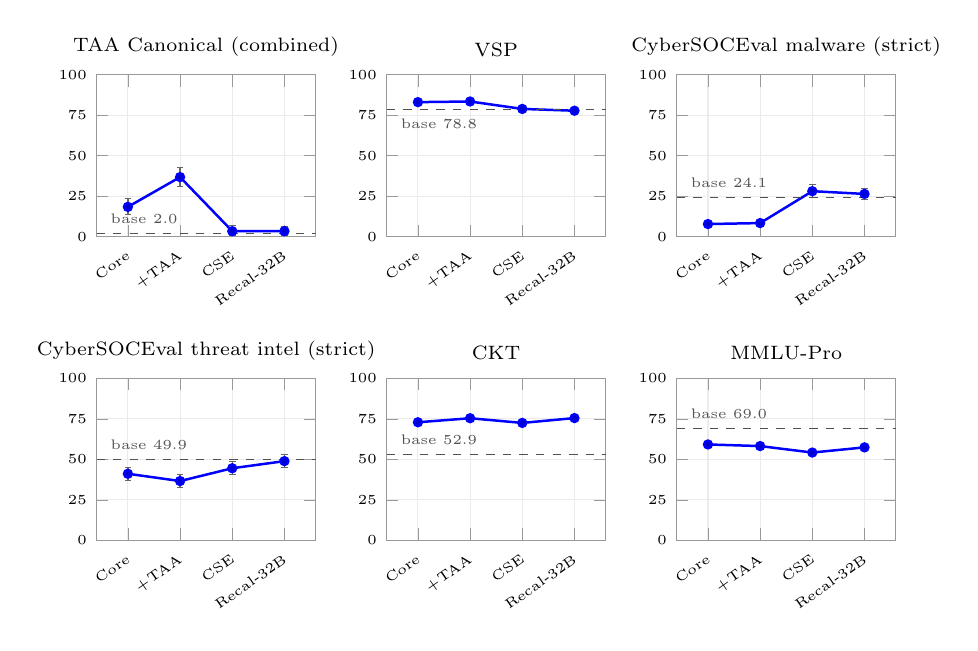
\begin{tikzpicture}
\begin{groupplot}[
  %% vertical sep must clear the rotated x tick labels of the upper row; at 13mm
  %% the lower row's titles printed on top of them.
  group style={group size=3 by 2, horizontal sep=9mm, vertical sep=18mm},
  width=0.36\textwidth, height=0.3\textwidth,
  ymin=0, ymax=100, ytick={0,25,50,75,100},
  xmin=-0.6, xmax=3.6, xtick={0,1,2,3}, xticklabels={Core,+TAA,CSE,Recal-32B}, x tick label style={font=\tiny, rotate=35, anchor=north east},
  y tick label style={font=\tiny}, title style={font=\scriptsize, yshift=-1mm},
  axis line style={black!40}, tick style={black!40}, grid=major, grid style={black!8},
  every axis plot/.append style={seriesblue, mark=*, mark size=1.4pt, line width=0.9pt, error bars/y dir=both, error bars/y explicit, error bars/error bar style={black!60, line width=0.5pt}, error bars/error mark options={black!60, rotate=90, mark size=1.2pt}}]
\nextgroupplot[title={TAA Canonical (combined)}]
\addplot coordinates {(0,18.4)+=(0,5.3)-=(0,4.9) (1,36.8)+=(0,5.7)-=(0,5.6) (2,3.4)+=(0,3.4)-=(0,2.6) (3,3.4)+=(0,3.0)-=(0,2.6)};
\draw[refgray, dashed] (axis cs:-0.6,2.0) -- (axis cs:3.6,2.0) node[pos=0.02, above right, font=\tiny, text=refgray] {base 2.0};
\nextgroupplot[title={VSP}]
\addplot coordinates {(0,83.1)+=(0,0.7)-=(0,0.7) (1,83.5)+=(0,0.6)-=(0,0.7) (2,78.9)+=(0,1.0)-=(0,1.0) (3,77.8)+=(0,1.1)-=(0,1.1)};
\draw[refgray, dashed] (axis cs:-0.6,78.8) -- (axis cs:3.6,78.8) node[pos=0.02, below right, font=\tiny, text=refgray] {base 78.8};
\nextgroupplot[title={CyberSOCEval malware (strict)}]
\addplot coordinates {(0,7.8)+=(0,2.3)-=(0,2.2) (1,8.4)+=(0,2.4)-=(0,2.2) (2,28.1)+=(0,4.1)-=(0,4.0) (3,26.4)+=(0,3.6)-=(0,3.5)};
\draw[refgray, dashed] (axis cs:-0.6,24.1) -- (axis cs:3.6,24.1) node[pos=0.02, above right, font=\tiny, text=refgray] {base 24.1};
\nextgroupplot[title={CyberSOCEval threat intel (strict)}]
\addplot coordinates {(0,41.1)+=(0,3.9)-=(0,4.0) (1,36.6)+=(0,3.8)-=(0,3.9) (2,44.5)+=(0,4.2)-=(0,4.1) (3,48.9)+=(0,4.1)-=(0,4.2)};
\draw[refgray, dashed] (axis cs:-0.6,49.9) -- (axis cs:3.6,49.9) node[pos=0.02, above right, font=\tiny, text=refgray] {base 49.9};
\nextgroupplot[title={CKT}]
\addplot coordinates {(0,72.9)+=(0,1.5)-=(0,1.6) (1,75.4)+=(0,1.6)-=(0,1.6) (2,72.5)+=(0,1.6)-=(0,1.6) (3,75.5)+=(0,1.6)-=(0,1.5)};
\draw[refgray, dashed] (axis cs:-0.6,52.9) -- (axis cs:3.6,52.9) node[pos=0.02, above right, font=\tiny, text=refgray] {base 52.9};
\nextgroupplot[title={MMLU-Pro}]
\addplot coordinates {(0,59.2)+=(0,0.9)-=(0,0.8) (1,58.2)+=(0,0.9)-=(0,0.9) (2,54.2)+=(0,0.9)-=(0,0.9) (3,57.4)+=(0,1.0)-=(0,0.9)};
\draw[refgray, dashed] (axis cs:-0.6,69.0) -- (axis cs:3.6,69.0) node[pos=0.02, above right, font=\tiny, text=refgray] {base 69.0};
\end{groupplot}
\end{tikzpicture}
\caption{Six task scores across the retained checkpoints of the canonical chain (points) with 95\% item-bootstrap intervals (bars) and the base model's score as a dashed reference. Intervals for the base are not available. The panels share one 0--100 axis; Stage 3 (CSE) raises the SOC-style tasks and collapses canonical attribution and part of VSP, and Stage 4 recovers CKT and MMLU-Pro but neither attribution nor VSP.}\label{fig:trajectories}
\end{figure}

\begin{table}[!htbp]
\centering\scriptsize
\setlength{\tabcolsep}{3.5pt}
\caption{Paired differences between checkpoints (later minus earlier) with 95\% paired item-bootstrap intervals; intervals that exclude zero are marked with an asterisk. These quantify item-sampling uncertainty for the specific trained models, not training-seed variance.}\label{tab:paired}
\fitwidth{\begin{tabular}{@{}lrrrr@{}}
\toprule Metric & +TAA $-$ Core & CSE $-$ +TAA & Recal-32B $-$ CSE & Recal-32B $-$ Core \\\midrule
CKT & $+2.6$ \ci{+1.0}{+4.2}* & $-3.0$ \ci{-4.5}{-1.4}* & $+3.1$ \ci{+1.5}{+4.6}* & $+2.7$ \ci{+1.1}{+4.2}* \\
ATE & $-3.8$ \ci{-7.6}{+0.2} & $0.0$ \ci{-4.8}{+4.6} & $+2.4$ \ci{-2.4}{+7.2} & $-1.4$ \ci{-5.2}{+2.8} \\
RCM & $-0.8$ \ci{-1.3}{-0.2}* & $-1.3$ \ci{-2.2}{-0.4}* & $-0.6$ \ci{-1.9}{+0.8} & $-2.7$ \ci{-3.9}{-1.5}* \\
RMS & $-1.0$ \ci{-3.3}{+1.6} & $+0.9$ \ci{-1.5}{+3.3} & $-1.2$ \ci{-3.9}{+1.5} & $-1.3$ \ci{-4.0}{+1.4} \\
VSP & $+0.3$ \ci{-0.1}{+0.7} & $-4.5$ \ci{-5.5}{-3.5}* & $-1.1$ \ci{-2.3}{0.0} & $-5.3$ \ci{-6.4}{-4.2}* \\
TAA Classic & $+0.5$ \ci{-5.0}{+6.0} & $+6.5$ \ci{+1.0}{+12.5}* & $-3.0$ \ci{-8.5}{+2.5} & $+4.0$ \ci{-1.5}{+9.5} \\
TAA Canonical & $+18.4$ \ci{+12.4}{+24.4}* & $-33.5$ \ci{-39.8}{-27.1}* & $0.0$ \ci{-3.0}{+2.6} & $-15.0$ \ci{-20.7}{-9.4}* \\
CSE malware (strict) & $+0.6$ \ci{-0.4}{+1.6} & $+19.7$ \ci{+15.3}{+24.2}* & $-1.8$ \ci{-4.5}{+1.0} & $+18.6$ \ci{+14.9}{+22.5}* \\
CSE threat intel (strict) & $-4.5$ \ci{-6.7}{-2.3}* & $+7.9$ \ci{+3.3}{+12.4}* & $+4.4$ \ci{+1.8}{+7.2}* & $+7.9$ \ci{+3.6}{+12.0}* \\
CyberMetric 10K & $-0.3$ \ci{-0.6}{0.0} & $-0.3$ \ci{-0.7}{+0.1} & $+0.8$ \ci{+0.5}{+1.2}* & $+0.2$ \ci{-0.2}{+0.6} \\
MMLU-Pro & $-1.0$ \ci{-1.7}{-0.4}* & $-4.0$ \ci{-4.8}{-3.2}* & $+3.2$ \ci{+2.5}{+3.9}* & $-1.8$ \ci{-2.6}{-1.1}* \\
$\Abal$ & $+1.1$ \ci{+0.1}{+2.2}* & $-3.6$ \ci{-4.8}{-2.3}* & $+0.2$ \ci{-0.9}{+1.3} & $-2.3$ \ci{-3.4}{-1.1}* \\
$\Bbal$ & $-0.1$ \ci{-0.6}{+0.4} & $+2.7$ \ci{+1.7}{+3.8}* & $+0.6$ \ci{-0.2}{+1.4} & $+3.2$ \ci{+2.2}{+4.2}* \\
\bottomrule
\end{tabular}}
\end{table}

Stage 3 raises CyberSOCEval malware strict accuracy by 19.7 points and threat-intelligence accuracy by 7.9 relative to +TAA, but Canonical TAA falls by 33.5 points (interval $-39.8$ to $-27.1$), VSP by 4.5, CKT by 3.0, and MMLU-Pro by 4.0, all outside their intervals. Classic TAA rises by 6.5. Stage 3 also introduces parsing failures: 17.1\% of malware responses could not be parsed at the CSE checkpoint against 0.7\% at Core, and because the scorer excludes unparseable responses, the malware accuracy with failures counted as wrong is 23.3 rather than 28.1. The recovery stage does not meet its objective of restoring VSP: 77.8 is below both its CSE parent (78.9) and the base (78.8), and Canonical TAA stays at 3.4. It does recover CKT ($+3.1$), MMLU-Pro ($+3.2$), threat-intelligence accuracy ($+4.4$), and both CyberMetric tiers, and it lowers the malware parsing-failure rate to 5.9\%. The resulting $\Bbal$ increase of 0.6 has an interval that includes zero.

The label ``ship'' in the project denotes the released checkpoint, not a statistically established optimum. Relative to the CSE parent, the 14B-derived recipe loses 3.3 VSP points (interval $-4.4$ to $-2.2$) where the 32B-specific recipe loses 1.1; in a direct paired comparison the 32B-specific recipe is better on VSP ($+2.2$, interval $+1.0$ to $+3.4$), ATE ($+4.2$, $+0.2$ to $+8.2$), and MMLU-Pro ($+2.8$, $+2.1$ to $+3.4$), and worse on nothing beyond noise; the aggregate difference of 0.4 $\Bbal$ points has an interval that includes zero. Both are single training runs, so repeated seeds under a frozen selection rule are still needed to distinguish a robust recipe effect from training stochasticity.

\subsection{Why canonical attribution collapses}
Aggregate scores cannot distinguish a loss of attribution knowledge from an output-format change, so we classified every Canonical-TAA response of the five checkpoints (Table~\ref{tab:taataxonomy}). The collapse is not a parsing artifact. At the CSE checkpoint every response is well-formed and 124 of 133 name a real ATT\&CK group that is the wrong one; the model also stops emitting G-codes altogether, which returns at Stage 4 without restoring correctness. The gain at +TAA is likewise instructive: 64 of its 133 responses name another known alias of the correct group rather than the canonical name, and receive half credit. The task therefore measures alias normalization on top of association knowledge, and the SOC-oriented stage overwrote the association. Classic TAA shows a different profile: roughly 70\% of responses at every checkpoint receive half credit for a related group, so its combined score is dominated by plausibility credit rather than exact attribution.

\begin{table}[!htbp]
\centering\footnotesize
\caption{Response taxonomy for the 133 Canonical-TAA items. ``Known group'' means the predicted name is in the benchmark's alias table. Rows sum to 133; the last line counts responses containing an ATT\&CK G-code.}\label{tab:taataxonomy}
\fitwidth{\begin{tabular}{@{}lrrrrr@{}}
\toprule Outcome & Core & +TAA & CSE & Recal-14B & Recal-32B \\\midrule
Strict match (canonical name or G-code) & 9 & 17 & 4 & 5 & 3 \\
Another alias of the correct group (half credit) & 31 & 64 & 1 & 5 & 3 \\
Wrong but known group & 78 & 32 & 124 & 108 & 113 \\
Name not in the alias table & 7 & 2 & 4 & 10 & 14 \\
Missing final answer line & 8 & 18 & 0 & 5 & 0 \\\midrule
Responses containing a G-code & 113 & 132 & 0 & 126 & 121 \\\bottomrule
\end{tabular}}
\end{table}

\subsection{Where the severity regression comes from}
VSP is scored by base-score distance, so a checkpoint can score 77.8 while matching the exact eight-metric vector in only 13.6\% of items. Table~\ref{tab:vsp} decomposes mismatches by CVSS metric. Exact-vector agreement falls from 25.6\% at +TAA to 16.4\% at CSE and 13.6\% at the final checkpoint. The regression is concentrated in the exploitability metrics: mismatches on Privileges Required more than double (357 to 799 items), Attack Vector quadruples (136 to 537), and Scope nearly quadruples (115 to 421), whereas the impact metrics (confidentiality, integrity, availability) are unchanged or slightly better. The SOC-oriented stage therefore shifted the model's judgment of how a vulnerability is reached rather than what it affects, which the distance-based score partly masks. A metric-level score should accompany the base-score distance in future reporting.

\begin{table}[!htbp]
\centering\footnotesize
\caption{VSP error profile over 2,000 items: exact-vector matches and number of items mismatching each CVSS v3.1 base metric.}\label{tab:vsp}
\fitwidth{\begin{tabular}{@{}lrrrrrrrrr@{}}
\toprule Checkpoint & Exact vector & AV & AC & PR & UI & S & C & I & A \\\midrule
Core & 483 (24.2\%) & 149 & 127 & 369 & 344 & 163 & 634 & 653 & 341 \\
+TAA & 513 (25.6\%) & 136 & 131 & 357 & 342 & 115 & 618 & 661 & 340 \\
CSE & 329 (16.4\%) & 537 & 125 & 799 & 422 & 421 & 578 & 504 & 356 \\
Recal-14B & 305 (15.2\%) & 556 & 126 & 774 & 392 & 405 & 520 & 489 & 420 \\
Recal-32B & 271 (13.6\%) & 583 & 211 & 791 & 372 & 525 & 601 & 507 & 444 \\\bottomrule
\end{tabular}}
\end{table}

\subsection{Qualitative schema examples}
Three items from the retained artifacts illustrate how individual mapping errors change between Core and the final checkpoint; they are illustrations, not a representative error sample. For ATE item 38 (stolen SSH credentials used to log into a Linux build server), Core answered T1078 (Valid Accounts) and the final checkpoint answered T1021.004 (Remote Services: SSH), which the parent-level scorer credits against the gold T1021.004 even though the prompt asked for a parent technique. For RCM item 10 (local unauthenticated file tampering in MicroSCADA X SYS600), the answer changed from CWE-732 to the gold CWE-276 (Incorrect Default Permissions). For CKT item 15 (the Tangelo mobile malware's audio-capture capability), the answer changed from option C (T1533) to the gold option B (T1429, Audio Capture). Full prompts and responses are in the released artifacts.

\subsection{Cross-architecture ports}
Table~\ref{tab:ports} reports the selected checkpoint of each port under the uniform aggregation, with the corresponding base. The dense Qwen ports gain on every aggregate and lose 11.6 to 13.9 MMLU-Pro points. The MoE port gains 1.6 points on $\Bbal$ and 6.0 on the ten-test mean but loses 24.6 MMLU-Pro points; its base was evaluated with thinking mode enabled while the fine-tuned checkpoints were served without it, so that comparison mixes a serving change with the training effect. The two 8B ports are negative findings under the three-benchmark mean: Foundation-Sec-8B, an already security-specialized base, loses 2.9 points on $\Bbal$ despite a 0.4-point gain on the ten-test mean, and Llama-3.1-8B loses 0.9 points, in both cases because CyberMetric drops by nine to thirteen points. Applying the same recipe to an already specialized or much smaller base is not recommended without architecture-specific tuning. Differences in pretraining, the adapted Stage-4 recipe, and serving behavior prevent a clean size-only conclusion.

\begin{table}[!htbp]
\centering\footnotesize
\caption{Cross-architecture ports under the uniform aggregation: base model versus the port's selected checkpoint. Selection is the project's release designation. All values are single evaluations from the consistent sheet of the results workbook.}\label{tab:ports}
\fitwidth{\begin{tabular}{@{}llrrrrrrrrr@{}}
\toprule & & \multicolumn{3}{c}{$\Bbal$} & \multicolumn{3}{c}{Ten-test mean} & \multicolumn{3}{c}{MMLU-Pro} \\\cmidrule(lr){3-5}\cmidrule(lr){6-8}\cmidrule(lr){9-11}
Base model & Checkpoint & base & port & $\Delta$ & base & port & $\Delta$ & base & port & $\Delta$ \\\midrule
Qwen2.5-32B-Instruct & Recal-32B & 57.7 & 65.0 & $+7.3$ & 49.6 & 62.9 & $+13.3$ & 69.0 & 57.4 & $-11.6$ \\
Qwen2.5-14B-Instruct & Recalibrate & 55.1 & 61.0 & $+5.9$ & 46.1 & 59.6 & $+13.5$ & 64.1 & 50.2 & $-13.9$ \\
Qwen3-30B-A3B-Thinking$^{a}$ & CSE & 61.8 & 63.4 & $+1.6$ & 54.9 & 60.9 & $+6.0$ & 77.6 & 53.0 & $-24.6$ \\
Foundation-Sec-8B-Instruct & Recalibrate & 56.4 & 53.5 & $-2.9$ & 52.7 & 53.2 & $+0.4$ & 43.2 & 25.6 & $-17.6$ \\
Llama-3.1-8B-Instruct & Recalibrate & 50.7 & 49.8 & $-0.9$ & 43.4 & 50.8 & $+7.3$ & 48.3 & 27.7 & $-20.6$ \\\bottomrule
\end{tabular}}\par\smallskip
{\scriptsize $^{a}$Base evaluated with thinking mode enabled; fine-tuned checkpoints served without it. Stage 4 was closed for this port because neither recipe beat the CSE checkpoint.\par}
\end{table}

\subsection{Hosted reference models}
Table~\ref{tab:frontier} places the final checkpoint among hosted references evaluated with the same harness. Because the hosted rows were always computed with $\Tbal$, they are directly comparable with the corrected local rows. The final checkpoint is 7.9 points below GPT-5.5, 5.4 below DeepSeek-V4-Pro, 4.8 below Gemini-3-Flash-Preview, 2.5 below GPT-5.2, 1.0 below DeepSeek-V3.2-Exp, and 1.6 above Gemini-2.5-Flash on $\Bbal$; on the ten-test mean it is between GPT-5.2 and DeepSeek-V3.2-Exp. Its AthenaBench score is within five points of the second-ranked hosted model, while its CyberSOCEval composite ties the base for the lowest value in the table and its MMLU-Pro score is 20 to 30 points below every hosted reference. The hosted evaluations are single runs whose run manifests were not re-audited here, and model versions and reasoning settings are those recorded at evaluation time.

\begin{table}[!htbp]
\centering\footnotesize
\caption{Hosted references and the local models under the uniform aggregation (single evaluations; hosted rows as recorded in the results workbook). GPT-5.2 was run at medium reasoning effort.}\label{tab:frontier}
\fitwidth{\begin{tabular}{@{}lrrrrrr@{}}
\toprule Model & $\Abal$ & $C$ & $Y$ & $\Bbal$ & Ten-test mean & MMLU-Pro \\\midrule
GPT-5.5 & 77.0 & 48.3 & 93.3 & 72.9 & 73.5 & 88.3 \\
DeepSeek-V4-Pro & 67.2 & 52.2 & 91.8 & 70.4 & 67.9 & 79.1 \\
Gemini-3-Flash-Preview & 69.3 & 48.1 & 92.1 & 69.8 & 68.4 & 89.2 \\
GPT-5.2 & 63.8 & 46.8 & 91.9 & 67.5 & 65.0 & 81.3 \\
DeepSeek-V3.2-Exp & 59.0 & 47.2 & 91.7 & 66.0 & 62.2 & 82.5 \\
Glaukopis Recal-32B (this work) & 62.6 & 42.6 & 89.8 & 65.0 & 62.9 & 57.4 \\
Gemini-2.5-Flash & 53.1 & 46.2 & 91.1 & 63.4 & 57.9 & 82.1 \\
Qwen2.5-32B-Instruct (base) & 40.3 & 42.6 & 90.2 & 57.7 & 49.6 & 69.0 \\\bottomrule
\end{tabular}}
\end{table}

\section{Evaluation expenditure and lifecycle economics}\label{sec:cost}
\subsection{Recorded expenditure is not cost per pass}
The project's cost ledger combines hosted-API token accounting with local elapsed-time accounting at an assumed \$2.50 per GPU-hour on a two-H100 host \citep{glaukopis2026software}. Commercial API charges and local compute rental are different economic quantities, and neither includes all costs of operating a production SOC assistant. The audit found two accounting boundaries that the earlier draft did not report. First, the API accounting restores and accumulates token counters across reruns, so a hosted total can include repeated or partial passes; the run records needed to separate them were not available to us. Second, the local aggregator sums elapsed time over every summary file in a model's directory, which includes a model-level summary that repeats every task, so every local row of the ledger is exactly twice the elapsed time of the underlying runs. We verified this against the per-suite run manifests of all five 32B checkpoints; for the base model and the other ports only the ledger values exist locally.

\subsection{Single-pass and CTI-only expenditure}
Table~\ref{tab:cost} therefore reports, for the five audited checkpoints, the single-pass cost recomputed from the run manifests, and for all other rows the ledger values with their known limitations. The final checkpoint's full evaluation suite took 1,020 seconds on two H100 GPUs, or \$1.42 at the assumed rate, of which the three CTI benchmarks account for \$1.02 and MMLU-Pro for \$0.39. Among the hosted references, MMLU-Pro dominates the ledger for the reasoning-heavy models (87\% of Gemini-3-Flash-Preview's total), so the choice to include a general-task diagnostic materially changes any cost comparison. On the CTI portion alone, the recorded hosted expenditures range from about 4 times (DeepSeek-V3.2-Exp) to about 314 times (GPT-5.5) the final checkpoint's single-pass cost. These are expenditure ratios under the stated accounting bases, not controlled per-query prices, and they compare models of different capability.

\begin{table}[!htbp]
\centering\footnotesize
\caption{Evaluation expenditure in USD. Hosted rows are API token ledgers that may include reruns. Local rows marked ``run record'' are single passes recomputed from the per-suite run manifests (two H100 GPUs at \$2.50 per GPU-hour); the ledger value, which double-counts every task, is shown in parentheses. CTI-only is AthenaBench + CyberSOCEval + CyberMetric. No training cost is included.}\label{tab:cost}
\fitwidth{\begin{tabular}{@{}llrrrrr@{}}
\toprule Model & Basis & AthenaBench & CyberSOCEval & CyberMetric & MMLU-Pro & CTI-only / total \\\midrule
Gemini-3-Flash-Preview & API ledger & 5.72 & 78.46 & 64.46 & 1,005.49 & 148.64 / 1,154.13 \\
GPT-5.5 & API ledger & 202.62 & 79.19 & 38.73 & 187.60 & 320.53 / 508.13 \\
GPT-5.2 & API ledger & 30.44 & 23.28 & 4.04 & 151.90 & 57.77 / 209.67 \\
Gemini-2.5-Flash & API ledger & 56.68 & 12.26 & 19.08 & 78.23 & 88.01 / 166.24 \\
DeepSeek-V4-Pro & API ledger & 0.32 & 27.93 & 9.87 & 88.28 & 38.12 / 126.40 \\
DeepSeek-V3.2-Exp & API ledger & 0.01 & 3.68 & 0.45 & 7.10 & 4.14 / 11.24 \\\midrule
Qwen2.5-32B-Instruct (base) & local ledger$^{a}$ & 2.54 & 0.61 & 0.23 & 7.29 & 3.38 / 10.67 \\
Core & run record & 0.53 & 0.33 & 0.12 & 0.47 & 0.98 / 1.44 (2.88) \\
+TAA & run record & 0.49 & 0.33 & 0.11 & 0.43 & 0.93 / 1.36 (2.73) \\
CSE & run record & 0.37 & 0.29 & 0.11 & 0.31 & 0.77 / 1.09 (2.18) \\
Recal-14B & run record & 0.52 & 0.29 & 0.12 & 0.32 & 0.93 / 1.25 (2.51) \\
Recal-32B & run record & 0.61 & 0.30 & 0.12 & 0.39 & 1.02 / 1.42 (2.83) \\\bottomrule
\end{tabular}}\par\smallskip
{\scriptsize $^{a}$Ledger value; run manifests for the base were not available. If the same double count applies, the single-pass values are half of those shown.\par}
\end{table}

The base model's ledger entry is notable for a different reason: its MMLU-Pro evaluation cost 7.29 against 0.39 for the final checkpoint, because the base produces long reasoning outputs where the fine-tuned model answers tersely. Part of the local model's apparent inference economy is therefore a change in response length, which is also a plausible contributor to its lower MMLU-Pro score.

\subsection{Training amortization and break-even conditions}
For a fixed workload definition and acceptable quality level, let $C_{\mathrm{fixed}}$ include graph construction, corpus generation, the successful training chain, and setup costs, and report exploratory or failed runs separately. The training component requires per-pass GPU-hours and rates:
\begin{equation}
 C_{\mathrm{train}}=\sum_s g_s h_s r_s,
\end{equation}
where $g_s$ is the GPU count, $h_s$ the elapsed training hours, and $r_s$ the cost per GPU-hour. The project's documented wall-time budget for the canonical chain is 51--64 hours on eight H100 GPUs (Table~\ref{tab:training}), or 408--512 GPU-hours; at the same \$2.50 rate that is \$1,020--\$1,280 for one successful chain, excluding data construction, failed or exploratory runs, and evaluation. This is a planning figure, not a metered bill.

For $N$ comparable workloads, write $C_{\mathrm{local}}(N)=C_{\mathrm{fixed}}+C_{\mathrm{maint}}(N)+Nc_L$ and $C_{\mathrm{API}}(N)=Nc_A$, where $c_L$ and $c_A$ must be measured on the same task population under stated serving conditions. If maintenance is negligible or already included, the first workload count at which local cost is no greater than API cost is
\begin{equation}
 N_{\mathrm{BE}}=\left\lceil\frac{C_{\mathrm{fixed}}}{c_A-c_L}\right\rceil,\qquad c_A>c_L,
\end{equation}
and there is no finite break-even if $c_A\le c_L$. Taking the CTI evaluation suite as the workload unit and the values of Table~\ref{tab:cost} at face value, $c_A-c_L$ is \$3.12 for DeepSeek-V3.2-Exp and \$319.51 for GPT-5.5, so the training budget alone would be recovered after roughly 330--410 suite-equivalents against the former and four against the latter. The two comparisons bracket very different capability levels, the API figures may include reruns, and standing capacity, utilization, staff time, electricity, refresh training, and depreciation are omitted; the equations, not these illustrative counts, are the claim.

\section{Threats to validity and operational boundaries}\label{sec:limits}
The first threat is attribution of benefit. Graph-derived data, shard composition, training duration, order, and hyperparameters co-vary. The present record demonstrates observable transitions with item-level uncertainty, not superiority over matched monolithic instruction tuning. A Core$\rightarrow$CSE control would test the need for the attribution stage; an equal-token mixed-data control would test the scheduling hypothesis; a data-provenance ablation would be required to quantify the contribution of Sophia independently of scheduling.

The second threat is evaluation alignment and selection. Section~\ref{sec:overlap} shows that exact gold-fact overlap does not inflate the mapping scores, but public-catalog overlap, common answer spaces, unscreened auxiliary data, incomplete verbatim-screen coverage, and repeated benchmark-guided recipe development limit an out-of-sample interpretation. A defensible extension would freeze a training graph, select checkpoints on separate development data, and evaluate once on a later, independently constructed incident set with documented entity and fact exclusions.

The third threat is uncertainty. The bootstrap intervals cover item sampling for the specific trained models; they do not cover training-seed variance, and they treat clustered items as independent. Several independently seeded Stage-4 runs would test the narrow recipe-selection question; seeded replication of the whole chain would be needed for the stage-effect claims. No significance test beyond the paired intervals is reported.

The fourth threat is the distinction between catalog competence and operational safety. An 11.6-point MMLU-Pro decrease at 32B and larger losses on other ports motivate explicit workload boundaries. The final Canonical-TAA score does not support autonomous actor attribution, and the VSP error profile shows systematic exploitability misjudgement after Stage 3. The model should not be the sole basis for high-consequence attribution, incident containment, unrestricted tool execution, legal advice, or decisions requiring broad reasoning outside the validated CTI schemas. Prompt-injection resistance, private-telemetry performance, latency under concurrent load, and human-analyst utility have not been established.

Finally, source-relative auditability is distinct from repeatability, reproducibility, and correctness. Replaying generation requires immutable graph and template snapshots; reproducing training also requires the actual rows, seeds, environment, and optimizer settings; reproducing evaluation requires complete inputs, outputs, scoring code, and run boundaries. The retained per-item artifacts and run manifests used here satisfy the last requirement for the five fine-tuned checkpoints but not for the base model or the hosted references.

\section{Conclusion}\label{sec:conclusion}
Glaukopis provides a concrete mechanism for constructing source-resolvable CTI instruction targets and observing specialization across retained checkpoints. After re-deriving every figure from the primary artifacts, the canonical 32B results show large improvements in attack-technique extraction, mitigation scoring, and CTI knowledge, a three-benchmark mean of 65.0 against 57.7 for the base under a uniform attribution convention, and pronounced interference: canonical attribution collapses after the SOC-oriented stage through wrong-but-well-formed group names, the severity regression concentrates in the exploitability metrics, and general-task performance declines. Item-level analysis shows that exact overlap between training rows and evaluation facts does not explain the mapping gains, while attribution and technique extraction track training exposure.

The evidence supports the graph-grounded data pipeline and the value of checkpoint-level diagnosis with quantified uncertainty. It does not yet establish that four-stage training is necessary or superior, that the gains extend to unseen enterprise incidents, or that recorded expenditure ratios constitute controlled lifecycle savings. Closing those gaps requires matched single-stage and skip-stage controls, seeded replication, and an entity-disjoint held-out incident set. Verifiable-reward training, as explored in related CTI work \citep{alam2026minerva}, is a possible extension but does not replace those controls.

\section*{CRediT authorship contribution statement}
\textbf{Peter J. Worth Jr.:} Conceptualization, Methodology, Software, Investigation, Data curation, Formal analysis, Writing -- original draft, Writing -- review \& editing. \textbf{Ionut Cardei:} Supervision, Methodology, Writing -- review \& editing. \textbf{Salman Ahmad:} Software, Validation, Data curation. \textbf{Muhammad Mamoon Khan:} Software, Data curation.
%% TODO (authors): confirm the roles of S. Ahmad and M. M. Khan before submission.

\section*{Declaration of competing interest}
This research was funded by Athena Security Group, LLC, which develops Glaukopis; P.~J.~Worth Jr.\ and I.~Cardei are affiliated with Athena Security Group. P.~J.~Worth Jr.\ and S.~Ahmad are co-authors of the AthenaBench benchmark used in the evaluation. These relationships are disclosed so that readers can assess the developer--evaluator overlap. The authors declare no other competing interests.

\section*{Funding}
This work was supported by Athena Security Group, LLC.

\section*{Data availability}
The Glaukopis software, training configuration, evaluation harness, cost aggregator, and the results workbook are available in the project repository at commit \code{c4d3a2f45e0a08672c87c2b46c3c4be109440c38} under the PolyForm Noncommercial 1.0.0 license \citep{glaukopis2026software}; the repository is source-available, not open-source. The final and intermediate checkpoints are documented at \url{https://huggingface.co/asg-ai}. The per-item prediction and score files for the five fine-tuned checkpoints, the build reports of the contamination screen, and the analysis scripts that produce every table and interval in this article (bootstrap, error taxonomies, entity overlap, cost recomputation) are provided as supplementary material.
%% TODO (authors): deposit the supplementary package (per-item artifacts, build reports, analysis/ scripts) in a persistent archive and insert the DOI.

\section*{Declaration of generative AI and AI-assisted technologies in the writing process}
During the preparation of this work the authors used OpenAI ChatGPT and Anthropic Claude Code in order to restructure and edit the manuscript text, check bibliographic records, and draft the arithmetic-verification and item-level analysis scripts that accompany the manuscript. After using these tools, the authors reviewed and edited the content as needed and take full responsibility for the content of the published article.

\bibliographystyle{elsarticle-harv}
\bibliography{glaukopis_cs_v1.5}

\end{document}
